\section{System Design}
\label{sec:system}


\subsection{Design Overview}
\label{sec:overview}
\begin{figure}[h]
    \centering
    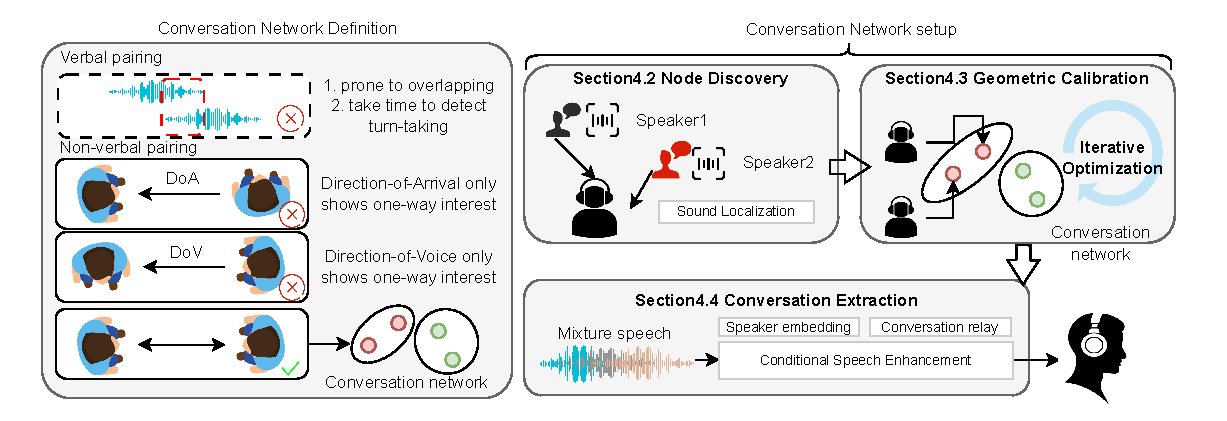
\includegraphics[width=1\linewidth]{chapters/cohear/figs/overview.pdf}
    \vspace{-1em}
    \caption{Overview of the CoHear system. We conduct node discovery for each user and carry out geometric calibration collaboratively. Finally, we perform target conversation extraction based on clues related to the members of the conversation.}
    \label{fig:system overview}
    \vspace{-1em}
\end{figure}

CoHear is a novel network system specifically designed to establish connections based on conversational features, as illustrated in Fig. \ref{fig:system overview}. To achieve this, we define a "conversation network" as the foundation of the system, where individuals participating in the same conversation will experience conversation enhancement.
To construct such a network, the first step is to define its basic components: pairings and which participants are considered part of the same conversation. The details of this definition will be discussed in the next subsection.
Given the definition of the conversation network, the next step is to implement it in the real world using earphones, as shown on the right side of Fig. \ref{fig:system overview}. CoHear employs a two-stage process for conversation modeling. In the first stage, we set up the conversation through acoustic sensing and optimization, and in the second stage, we perform enhancement powered by the network.

The implementation consists of three core components:
First, the \textbf{node discovery} module acts as the front end of our system, where nearby nodes (i.e., speakers) are identified using deep learning-based sound source localization. We extract both the locations and embeddings of each speaker to serve as input for the next stage. Note that this process applies to all speakers wearing earphones; further details are provided in Sec. \ref{sec:acoustic}.
Second, \textbf{geometric calibration} is performed in a centralized manner by aggregating the outputs of the node discovery module from each speaker, as discussed in Sec. \ref{sec:geometric}. Although each node can only observe others within its local coordinate system, we iteratively optimize a shared global geometry. The more observations we obtain from the speakers, the more stable the optimization becomes. After completing the initial optimization with a cold start, we can track the speakers in real time.
Once the conversation network is established, the final component, \textbf{conversation enhancement}, performs conversation-level speech enhancement based on the identified participants (described in Sec. \ref{sec:conversation}). Specifically, both the speaker embedding (time-invariant) and the relay signal (time-variant) are used as cues for the conditional speech enhancement model. We introduce an audio control module to balance the contributions of these two approaches.

\paragraph{Conversational network}
To define our conversation network, the first step is answering the question: How can we technically model the conversation?'' Specifically, we break down a conversation into individual interactions performed by each participant, such as when user A speaks to user B. We observe that such a definition is similar to the concept of computer networking, where a sender sends pairing messages to find a receiver.
Accordingly, we construct a conversation network comprising all participants that can be successfully paired with the same conversation.
It is important to note that existing platforms, such as Livekit \cite{livekit}, provide real-time audio-visual sharing via WebRTC \cite{blum2021webrtc} Selective Forwarding Units (SFUs). In contrast, CoHear builds upon these platforms and extends their capabilities with advanced conversation modeling.

To enable the pairing of networks, we consider two features as discussed in Sec. \ref{sec:related}: verbal and non-verbal. Since the verbal feature (turn-taking) needs to wait for enough time before being effective, we consider the non-verbal feature as the main factor to determine the conversation.
We consider that a person's head orientation is a key indicator of their willingness to engage in conversation, both to speak and to listen. We define a conversation as requiring a bidirectional interest: individuals in the same conversational group must have an interest in at least one other person within the group. This mutual interest is depicted in the bottom left of Fig. \ref{fig:system overview}. As this pairing relies solely on non-verbal cues, we refer to it as the non-verbal pairing of a conversation network.
If we aim to implement this pairing using audio, sound source localization is a natural consideration. However, while sound source localization can estimate a person's relative position, it is insufficient for identifying conversational groups. This is because the DoA of sound can only determine a unidirectional interest (i.e., who is being listened to). Similarly, Direction-of-Voice also only indicates the other way of interest, so that both DoA and DoV are not the indicators for conversation.
Formally, combining both DoA and DoV allows us to infer the desired 6 Degrees of Freedom (6DoF) locations of participants. This necessity motivates us to move beyond the limitations of existing sound source localization methods.

Verbal features, such as turn-taking, serve as direct indicators of conversational engagement, as illustrated in the upper-left section of Fig. \ref{fig:system overview}. However, a significant drawback is their reliance on observing a sufficient duration of speech to be effective (i.e., one must wait for a turn-taking event to occur). Furthermore, overlapping audio is prone to interference from other speakers, which reduces reliability.
Consequently, the conversation network in our current implementation is primarily constructed using non-verbal pairing. Although these non-verbal features are also extracted from the audio signal—the same source as the verbal features—they are processed in a fundamentally different way. This alternative processing method ensures that the two aforementioned disadvantages do not apply to our design.


 


\begin{figure}[h]
    \centering
    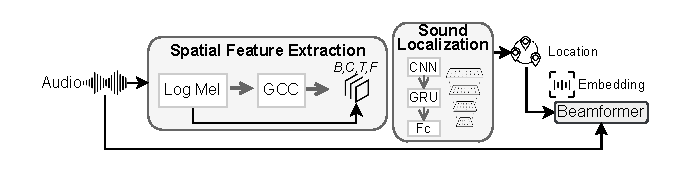
\includegraphics[width=0.7\linewidth]{chapters/cohear/figs/acoustic.pdf}
    \vspace{-1em}
    \caption{The node discovery for conversation setup: where we detect the sound source in the first stage and find the corresponding speaker embedding in the second stage.}
    \label{fig:acoustic}
    \vspace{-1em}
\end{figure}

\subsection{Node Discovery for Conversation Setup}
\label{sec:acoustic}
Conversation can be depicted through the interaction between speakers; the speaker presents the interest according to the direction of the voice (also the direction of the head). In CoHear, each user is considered as one node, where we reformulate speaker localization as a dynamic node discovery problem in a mobile acoustic network, as shown in Fig. \ref{fig:acoustic}. Specifically, it is necessary to access both the location and identity of the nearby nodes. We represent the location in local coordinates (the receiver as the root) and the identity as the voiceprint, which is an embedding that represents the voice of the speaker.

While joint estimation of these properties (similar to sound event localization and detection) is theoretically possible, prior work shows such approaches suffer from computational complexity and poor scalability \cite{wang2022nerc}. Instead, we adopt a decoupled two-stage discovery process that separately handles node localization and identity extraction and then fuses the results for network coordination.

\paragraph{Stage one: sound localization}
As for the sound localization, we extract the cross-channel features as Sec. \ref{sec:background} and utilize a convolutional recurrent neural network (CRNN) to process them, which consists of multiple convolutional layers, a GRU layer, and the final linear layer to predict the output. 
Specifically, we convert the multi-channel audio recording ($M \times T$) into multiple pairs of recordings ($N \times 2 \times T$), where $N$ refers to all the possible combinations. Then, we apply a log-mel spectrogram transformation for each channel and calculate GCC between every pair of channels. Lastly, we concatenate every pair of channels with the original log-Mel spectrograms as the final representations. For example, the feature has a shape of $(2+1) \times T \times F$ for two-channel audio recordings, which can be considered as the input to the neural network. As for the output format, we represent the sound source location in a cartesian coordinate system ($x, y, z$) with a normalized range of one meter radius ($x^2+y^2+z^2 = 1$), where the output dimension of the last linear layer is 3 with a tanh activation. When there is no sound source, the expected $x,y,z$ are set to zero. During inference, we only consider $x^2+y^2+z^2 > 0.5$ as a valid sound source.
Considering the output frame length is 0.1 seconds, we need to set the downsample ratio of the neural network to match it. Given the hop length of the spectrogram is 20ms, the time-dimension downsampling is set to 5. Consequently, the output format is $3 \times T/5$.

The above design only fits in one-source localization; we incorporate the multi-track \cite{cao2021improved} format for multi-source sound localization. Since we are only interested in the location rather than the sound class, the multi-ACCDOA \cite{shimada2022multi} format is unnecessary.
Considering the max number of sources is $n_{max}$, the output of the model is adjusted to $3*n_{max} \times T/5$ instead. Similar to sound separation, multi-source sound localization also needs permutation-invariant training as follows:
\(loss = \min_{\pi \in \Pi} (MSE(pred_\pi, gt))
\), where $\Pi$ refers to all the possible permutations of the sound sources, the above loss intends to find the optimal permutation (the least loss) and then perform back-propagation. 


\paragraph{Stage two: identity extraction}
After localizing all the sound sources, the next step is to associate the sound location with the identities. Although the speaker identities are accessible with the help of existing tools like Pyannotate \cite{bredin2023pyannote}, which supports overlapping speech and multiple speakers. 
However, the association between locations and identities can be difficult since they are two independent attributes. Specifically, the location of each person can be permuted randomly without impacting the results.

To associate them effectively, we can perform beamforming for each detected sound source and check which speaker's sound is amplified, which brings two subsequent problems: 1) how to perform beamforming with a limited microphone array, and 2) how to determine the identity of the beamformed speech. Although there are existing solutions for them respectively, directly combining them can lead to degradation since they are not co-optimized. 
For example, the output from beamforming can still contain noise, so that speaker identity extraction may not handle it well.

We propose a joint model to solve both the beamforming and embedding extraction at the same time. Specifically, we keep the beamformer (e.g., delay-and-sum beamformer) the same and reshape the output from \(B \times C \times T \times F\) to \(B \times T \times (F \times C)\) and use a linear projector with layer normalization to predict the d-vector. In addition, the final d-vector is the average over time. Since the output is not audio, we can not use the common loss function for neural beamformer (i.e., scale-invariant signal-noise ratio), but the cosine similarity loss as follows:
\(\text{L}(\mathbf{A}, \mathbf{B}) = 1- \frac{\mathbf{A} \cdot \mathbf{B}}{\|\mathbf{A}\| \|\mathbf{B}\|}\),
where \textit{A} is an estimated d-vector, and \textit{B} refers to the d-vector from clean speech with the speaker verification model.

In summary, the discovered node can be classified into three groups: self-voice, interested voice, and other voices. Note that the self-voice and interested voices come from a similar direction (i.e., the front of the user) with different distances, so it is hard to differentiate them with direction information only. Instead, we assume that the self-identity is given as prior knowledge, which is practical through offline or online enrollment. As a result, the self-voice can be identified by the similarity with the stored speaker embedding, so that we will not discover it as a new node.

\begin{figure}[h]
    \centering
    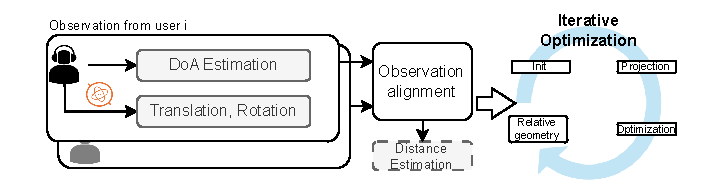
\includegraphics[width=0.7\linewidth]{chapters/cohear/figs/calibration.pdf}
    \vspace{-1em}
    \caption{Network geometric calibration uses the observed distance and direction of arrival, along with user motion, to estimate the locations of all users in the network via iterative optimization.}
    \label{fig:geometric_calibration}
    \vspace{-1em}
\end{figure}

\subsection{Network Geometric Calibration}
\label{sec:geometric}
As outlined in our system overview (Sec. \ref{sec:overview}), our ultimate goal is to estimate the positions of all users (nodes) in a conversation network. The previous node discovery step identifies nearby speakers, providing important positional observations. However, these outputs only indicate where people are speaking, not the structure of the conversation network itself. To achieve this, we propose aggregating observations from multiple participants to estimate the network's underlying geometry.
This task can be formulated as a multi-sensor localization problem, known as geometric calibration. Given that we use acoustic signals for localization, our approach falls within the category of WASN, as discussed in Section \ref{sec:background}.

This section details our geometric calibration pipeline. First, we describe how we obtain the necessary inputs: observation sharing and distance estimation, which provide DoA and distance measurements, respectively. Next, we introduce the concept of a Mobile WASN, distinguishing it from conventional Wireless Acoustic Sensor Networks. We then present our improved geometric calibration algorithm, which estimates the final positions of all nodes. Finally, we address two critical implementation factors: 1) reducing the warm-up time through dynamic calibration, and 2) enabling the system to operate with only a single device.

\paragraph{Observation alignment}
\label{sec:sharing}
The principle of geometric calibration is that one source can be observed by multiple nodes, where the relative position is related to the nodes' positions. Thus, it is important to align the source across nodes.
It is a trivial task when there is only one sound source, but it becomes complicated with 1) overlapping sound, 2) the sound isn't observed by some nodes. Since we have already extracted the corresponding speaker embedding for each source, we can assign the same identity to the sources with similar embeddings.
Specifically, for the speakers observed by one user (including itself), we pair all of them with the observations from other users and only keep the ones that have high similarity. The similarity is calculated by the cosine similarity of two embeddings.
A group of sources with more than 0.8 similarity is considered the same source. We don't make the assumption that one source can be observed by all users.
In practice, every device uploads its observed embeddings from Sec. \ref{sec:acoustic} to a central server and performs the above matching. Only the source that is observed by at least two nodes are considered as valid ones in the following.

\paragraph{Distance estimation}
\label{sec:distance}
According to the output of Sec. \ref{sec:acoustic}, we can only obtain the direction of arrival, while the distance to the sound source is skipped.
However, the distance information is important in geometric calibration since the optimization can be under-determined without it. Ideally, audio recordings already embed distance information in a reverberant environment, as illustrated in the following:
\[
y(t) = h(t) * x(t) + v(t) = h_{e}(t) * x(t) + h_{l}(t) * x(t) + v(t)
\], where \( v(t) \) corresponds to white sensor noise and \( h(t) \) represents the room impulse response, the symbol \( * \) denotes convolution. However, the performance highly relies on a known environment, so the scalability is not satisfying \cite{krause2021joint, gburrek2021geometry}.

Instead, we propose estimating distance by comparing the sound pressure levels at the transmitter and receiver. In an ideal scenario, the audio attenuation corresponds to the propagation path loss, which is related to distance. To ensure a clean input signal and mitigate the effects of multi-path propagation or overlapping sound sources, we selectively use audio segments containing only a single active source and compute the average sound level from these segments.
Despite this design, distance estimation errors may still be significant. Therefore, we do not use the estimated distance as a final output. Instead, we utilize it as an input for subsequent geometric calibration, alongside other data.



\paragraph{Mobile WASN}
According to Sec. \ref{sec:background}, our network can be considered as mobile WASN, an extension of WASN where the acoustic node can move freely. Similarly, localization of sensor nodes can be achieved by geometric calibration, given sufficient observed sound sources. Compared to the conventional notation, mobile WASN has different assumptions as follows.

\begin{enumerate}
    \item First, the assumption that only one sound source is present during a measurement is unrealistic due to the possibility of overlapping speech and other background sounds. Specifically, if we denote the maximum number of simultaneous speech sources as \(M\), we can estimate a total of \(M \times K \times L\) instances, which is also compatible with fewer than \(M\) number of sources by adding a blank estimate.
    \item Second, while all the estimates are considered valid in the previous context, the arbitrary movement of users can create a much greater distance between two sensor nodes, which means that some sound sources may not be observed by all sensor nodes.
    \item Third, the acoustic source \(S_{k}\) is defined as the \(k^{th}\) observed source during a specific time period. In this context, \(k\) (where \(k = 1, 2, \ldots, K\)) can also serve as a time identifier. The notation is important because we can align the sound source with the location of the sensor nodes, which are also time-dependent and can be represented as \(n_{k,l}\). Since the sensor nodes can move freely, we use \(T_{k,l}\) and \(R_{k,l}\) to indicate the translation and rotation between \(n_{k,l}\) and \(n_{0,l}\) for the \(l^{th}\) node.
    \item Lastly, it is expected that \(n_{k,l}\) will match at least one of the \(S_{k}\) since the sensor node is one of the sound sources. Note that it is not valid conversely since there are sound sources that come from people without earphones. 
\end{enumerate}


\paragraph{Geometric calibration}
We perform mobile geometric calibration with the networked earphones, which share a similar principle as other geometric calibrations that minimize a cost that is defined to evaluate how well these converted observations align with the assumed geometry. Among the various algorithms, data set matching is an efficient algorithm for geometric calibration. Our algorithm is based on that of \cite{gburrek2021geometry}; the details of it are out of the scope of this paper.. 

Different from the original algorithm, we have a rotation matrix \(R_{k,l}\) and a translation vector \(n_{k,l}\) that are dependent on both the source and the node. As a result, we rewrite the relative locations in the global coordinates:
\[
G_{k,l} = R_{k,l} d_{k,l} [cos(\theta_{k,l}), sin(\theta_{k,l})] + n_{k,l}
\]
Multiple nodes observe each source at the same time; if all the estimates are perfectly right, all \( S_{k,l}\) would map to a unique position \( G_{k,l} \). Hence, the geometry can be inferred by minimizing the deviation of the projected source positions by the cost function below:
\[
\arg\min \sum_{l=1}^{L} \sum_{k=1}^{K} \left\| G_{k,l} - S_{k,l} \right\|_2^2
\]
, where \( \| \cdot \|_2 \) denoting the Euclidean norm. There exists no closed-form solution for the above nonlinear optimization problem, so it has to be solved using an iterative optimization algorithm.

Compared to our setting, previous methods estimate 
\(R_{l}\) and translation \(n_{l}\) for L sensor nodes, while ours estimate \(K \times L\) nodes equivalently. The naive approach is performing geometric calibration for each source, downgrading to K times one source geometric calibration, and merging the results afterward.
According to the analysis in \cite{gburrek2021geometry}, the performance of geometric calibration depends on the number of sources. Consequently, the one-source geometric calibration will give unreliable results and harm the final performance.

Instead, we can further compose the translation into initial and movement: 
\(R_{k,l} = \overline{R}_{k,l}R_{0,l}\) and \(n_{k,l} = \overline{n}_{k,l} + n_{0,l}\), where \(\overline{R}_{k,l}\) refers the rotation from the first source to the k source for sensor l and \(\overline{n}_{k,l}\) refers the corresponding translation. We can see that if the \(\overline{R}_{k,l}\) is an identity matrix and \(\overline{n}_{k,l}\) is zero, the problem downgrades to the same as \cite{gburrek2021geometry}. As a result, we rewrite the above equation:
\[
G_{k,l} = R_{0,l} d_{k,l} \overline{R}_{k,l} [cos(\theta_{k,l}), sin(\theta_{k,l})] + \overline{n}_{k,l} +  n_{0,l}
\]
Fortunately, we can estimate \(\overline{R}_{k,l}\) and \(\overline{n}_{k,l}\) by a motion sensor on the node, which means our estimation targets become \(R_{0,l}\) and \(n_{0,l}\) so that the problem becomes estimating one locations instead of track. In other words, we can apply the data set match algorithm in the appendix.

In addition, the above processing can be generalized to multiple sources. Suppose \(M\) is the maximum number of simultaneous sources, the \(\overline{K}\) refers to the real number of sources within K times (\(K\leq\overline{K}\leq M \times K\)). We can set the \(R\) and \(n\) accordingly to fit in the original setting.

\paragraph{Dynamic calibration}
Based on our design, we conduct geometric calibration for every \(\overline{K}\) observation, which is not ideal for real-time inference. As a solution, we implement a sliding-window approach that allows us to repeat geometric calibration each time we receive new observations. Given that the runtime latency for this process is minimal, we plan to address the optimization in future work.

Meanwhile, selecting an optimal \(\overline{K}\) becomes critical, as it seems to be related to the latency and performance. Although the correlation between latency is obvious, the correlation with performance can be complicated. Specifically, the motion estimation (\(\overline{R}_{k,l}\) and \(\overline{n}_{k,l}\)) by IMU is also poisoned by accumulated errors with increasing \(\overline{K}\), which means the calibration may not be accurate with a large \(\overline{K}\). A small sliding window can be a direct solution to mitigate the degradation caused by noisy estimates. However, since the optimization needs sufficient observations to converge, the small window can conversely degrade the usability. Instead, we propose a weight decay algorithm where the calibration results focus more on the nearest observations. Specifically, we set the weight as \(  1/ (T-t)\), where \(T-t\) refers to the difference between the current time and the time of observations.

\paragraph{Single-device solution}
While collaborative calibration is the optimal approach, we propose a single-device method for scenarios where networking is impractical or latency is critical. In the evaluation, the above design will be considered as a special case when there is one earphone.
In geometric calibration, the output for each user is their position (\(P=(x_i, y_i)\))and orientation (\(O=\theta\)) within a shared coordinate system. However, in a single-user scenario, the shared coordinate system is defined relative to the user themself. In this case, the source's position and orientation relative to the user can be described by three key variables: the Direction of Arrival, the distance to the source, and the source's own orientation.

Assuming the sound source localization method from Section \ref{sec:acoustic} provides a reliable DOA, we note that the distance and source orientation variables are still missing. To address this, we modify our model to estimate these two additional variables.
Our neural network already outputs a 3-dimensional vector. We remove the unit vector constraint (\(x^2+y^2+z^2=1\)) to allow the model to represent sources at any distance. Furthermore, we add four additional output nodes to classify the sound source's orientation into one of four categories: front, left, right, or back. We use classification instead of regression for the orientation, as this challenging problem benefits from the increased stability that a classification approach provides.

\begin{figure}[h]
    \centering
    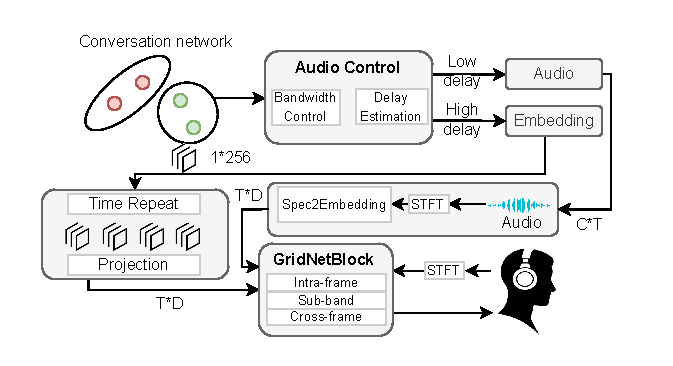
\includegraphics[width=0.7\linewidth]{chapters/cohear/figs/conversation_extraction.pdf}
    \vspace{-1em}
    \caption{Conversation extraction by target feature, which can be classified into time-invariant (speaker embedding) and time-variant. The adaptive audio control can balance the quality and bandwidth before sending to the neural network model.}
    \label{fig:voice_share}
    \vspace{-1em}
\end{figure}



\subsection{Conversation Extraction}
\label{sec:conversation}


\paragraph{Problem formulation}
For each group of nodes participating in the same conversation, the locations, identities (represented by speaker embeddings), and the audio recordings are shared among all members. We utilize this information to adjust the user's hearing (extract conversation) as demonstrated in Fig. \ref{fig:voice_share}.

Our design goal is to extract a target conversation from a speech mixture under specific conditions. While raw audio provides more fine-grained information than speaker embeddings, it consumes significantly more bandwidth. A naive solution, assuming we have access to a relatively clean audio relay, would be to transmit this audio directly like a video conference. However, this assumption is impractical for two reasons. First, even after noise suppression, we cannot guarantee that the transmitted audio perfectly matches the target speech. Second, the transmission process itself introduces delay, packet loss, and compression artifacts, resulting in a degraded version of the original received audio. Therefore, the core problem we address is how to design a conversation extraction model that can effectively utilize this degraded relay audio.

\paragraph{Adaptive audio control}
Ideally, relay audio should be transmitted at the highest possible quality. However, there will always be a bandwidth bound, particularly with multiple concurrent users. This is a common problem in networking, addressed by algorithms like TCP congestion control.
Unlike these well-established solutions, CoHear also considers the acoustic noise level, where a higher noise level indicates the need for a larger bandwidth (to provide more information as compensation). 
To achieve this, we can perform a grid search to maximize the overall conversation quality for all users under a total bandwidth constraint. For each user, we consider the distance as the indicator for conversation quality instead of directly estimating the metric like SNR. Consequently, the search objective is the sum of bandwidth/ distance for all the users within the conversation, where the total bandwidth is constrained. The reason behind our design is the close correlation between pair-to-pair distance and noise level.

Besides the bandwidth, transmission delay is another factor that needs consideration. Specifically, a delayed audio is almost useless even if he audio quality is good since the time-dimension correlation between the time-variant feature and the target speech diminishes, reducing its effectiveness as a reference. 
To address this, we propose estimating the transmission delay and disabling the time-variant feature when the latency exceeds a certain threshold. 
Specifically, we can utilize the GCC technique between the transmitted audio and the noisy speech, identifying the first peak as the delay.
Note that we don't need to estimate the delay frequently since we assume the delay is relatively stable.
In our empirical test, we find that a delay of 50ms is still tolerable for the time-variant feature and set it as the threshold.
Consequently, under poor network conditions, the system gracefully degrades by relying solely on time-invariant features for target speech extraction.
It is also important to note that the switch between time-invariant and time-variant features impacts bandwidth control. When audio transmission is not necessary (i.e., when the time-variant feature is disabled), the bandwidth requirement can be reduced accordingly.


\paragraph{Target conversation extraction}
Given the above analysis, the time-variant feature can be viewed as an extension of the time-invariant feature. Although the former provides richer information, several factors beyond bandwidth—such as latency, noise, and transmission losses (e.g., packet loss, bit errors)—can degrade the quality of these features.
Building on prior work in target speaker extraction \cite{veluri2024look}, we focus on target conversation extraction as an extension of speech enhancement. Existing target speech extraction methods typically rely on either time-invariant features, such as embeddings \cite{chen2024target, veluri2024look} or time-variant data like bone-conducted vibrations \cite{he2023towards}.
Time-invariant features, while compact and stable, can be viewed as ultra-highly compressed audio, potentially losing fine-grained details compared to time-variant data, like bone-conducted vibrations \cite{he2023towards} or relay audio \cite{shen2018mute}. To address this, CoHear is designed to strike a balance between compression and performance, optimizing both efficiency and accuracy.

Considering the time-invariant feature like speaker embedding, the enrollment speech (from the target user) is first converted to the speaker embedding by an encoder. To fit the feature in the model, the speaker embedding is projected to the same feature dimension and repeated to align with the time dimension. Lastly, the speaker embedding in the time-frequency dimension is added to the enhancement network. The pipeline is illustrated as follows:
\[
y = TSE(y_{noisy}, [e_{enrollment}, ....]_{T}), \quad e_{enrollment} = Embedder(y_{enrollment})
\], where the $TSE$ refers to the target speech extraction model (i.e., modified TFGridNet) and $Embedder$ refers to the speaker embedding extractor. We consider that $y_{enrollment}$ comes from the target user whose voice is mixed with noise in $y_{noisy}$.
As for the time-variant feature, which also refers to the target speech as the speaker embedding. We can transform the relay audio into a time-frequency feature using an STFT encoder. Similarly, the feature is added to the enhancement model, and the pipeline is illustrated below:
\[
y = TSE(y_{noisy}, [e_{enrollment}, ....]_{T}, E_{relay}), \quad E_{relay} = Embedder(y_{relay})
\]. To maintain compatibility with time-invariant features, we include both time-invariant features and time-variant features during the training by setting the features to zero when it is absent. Note that the actual form of the time-invariant feature is not the raw audio; we can further improve the efficiency by only transmitting the feature, and we leave it for future work. 
Besides, CoHear is expected to work well with multiple conditions (participants). A naive solution is to apply the speech filter multiple times, which is computation-intensive. Instead, we propose an attention mechanism that combines multiple conditions into the intermediate feature as follows: 
\(
 X = Attention([X_0, X_1, ...])
\)
, where \(X_i\) refers to the \(i^{th}\) conditions.







